\chapter*{Proposition 42}



\begin{figure*}[ht]
    \begin{center}
    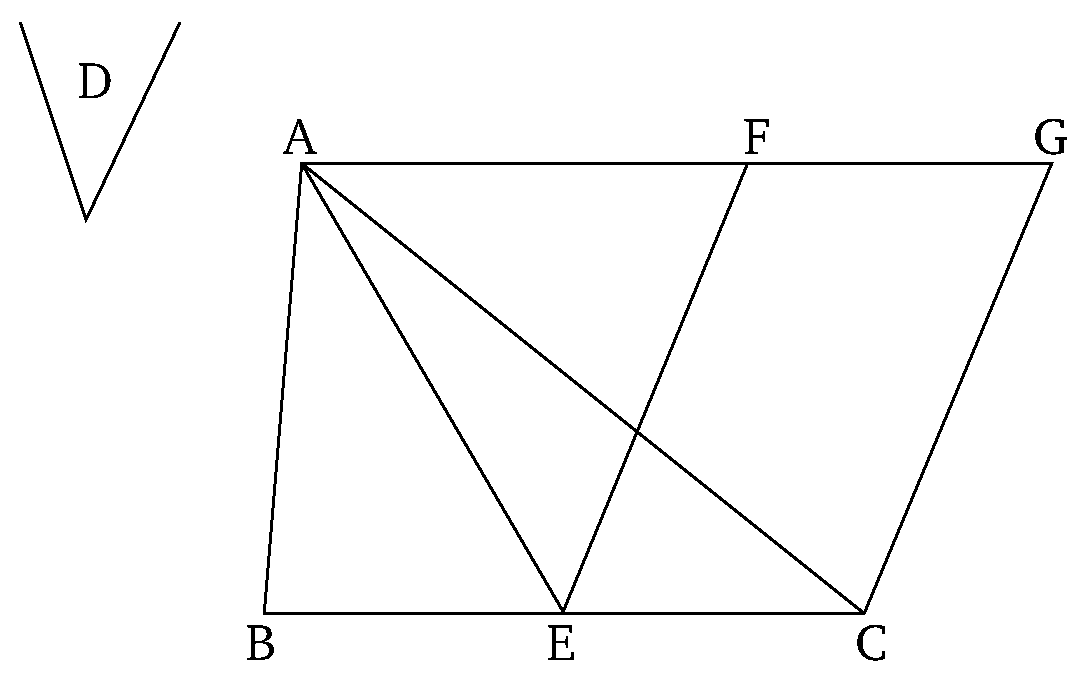
\includegraphics[width=0.5\linewidth]{figures/fig42e.eps}
    \label{fig:prop_42}
    \end{center}
\end{figure*}

To construct a parallelogram equal to a given triangle in a given
rectilinear angle.

Let $ABC$ be the given triangle, and $D$ the given rectilinear angle. So
it is required to construct a parallelogram equal to triangle $ABC$
in the rectilinear angle $D$.

Let $BC$ have been cut in half at $E$ [Prop.~1.10], and let $AE$ have been joined. And let (angle) $CEF$, equal to angle $D$,  have been constructed
at the point $E$ on the straight-line $EC$ [Prop.~1.23]. And let $AG$ have been drawn through $A$
parallel to $EC$ [Prop.~1.31], and let $CG$ have been drawn through $C$ parallel
to $EF$ [Prop.~1.31]. Thus, $FECG$ is a parallelogram. And since $BE$ is
equal to $EC$, triangle $ABE$ is also equal to triangle $AEC$. For they are
on the equal bases, $BE$ and $EC$, and between the same parallels, $BC$ and $AG$ [Prop.~1.38]. Thus, triangle $ABC$ is double (the area) of triangle $AEC$. And
parallelogram $FECG$ is also double (the area) of triangle $AEC$. For it has the same base as ($AEC$), and is between the same parallels  as ($AEC$) [Prop.~1.41].
Thus, parallelogram $FECG$ is equal to triangle $ABC$.  ($FECG$) also has
the angle $CEF$ equal to the given (angle) $D$.

Thus, parallelogram $FECG$,  equal to the given
triangle $ABC$, has been constructed in the angle $CEF$, which is equal to $D$. (Which is) the
very thing it was required to do.


\section*{Commentary}

\begin{proposition}\label{proposition_42}\lean{Elements.Book1.proposition_42}\leanok
    If
\end{proposition}
\begin{proof}
    \uses{proposition_10,proposition_23,proposition_31,proposition_38,proposition_41}\leanok
\end{proof}
